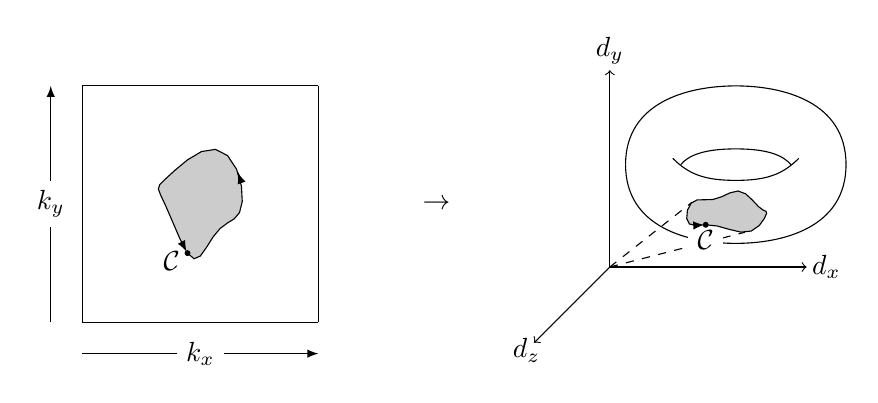
\begin{tikzpicture}

\def \axissize {2.5}
\def \squaresize{1.5}

\def \squarepos{-3}
\def \axisxpos {2.2}
\def \axisypos{-0.8}
\def \arrowdistance {0.4}

\draw (\squarepos - \squaresize , - \squaresize) -- (\squarepos + \squaresize, - \squaresize);
\draw (\squarepos + \squaresize , - \squaresize) -- (\squarepos + \squaresize, + \squaresize);
\draw (\squarepos + \squaresize , + \squaresize) -- (\squarepos - \squaresize, + \squaresize);
\draw (\squarepos - \squaresize , + \squaresize) -- (\squarepos - \squaresize, - \squaresize);

\draw [-latex] (\squarepos - \squaresize  , - \squaresize-\arrowdistance) -- (\squarepos + \squaresize, - \squaresize- \arrowdistance);
\draw [-latex] (\squarepos - \squaresize-\arrowdistance, - \squaresize) -- (\squarepos - \squaresize -\arrowdistance, + \squaresize) ;

\draw node [fill= white] at (\squarepos  , - \squaresize-\arrowdistance) {$k_x$};
\draw node [fill= white] at (\squarepos - \squaresize-\arrowdistance, 0)  {$k_y$};

\draw [-latex, fill= black!20, domain = 0:358] plot ({0.5 * (cos(\x-120) + 0.2 * sin(2*(\x-120))) + \squarepos},{0.6*(sin(\x-120) + 0.2 * cos(3*(\x-190))) });
\draw [-latex, domain = 160:161] plot ({0.5 * (cos(\x-120) + 0.2 * sin(2*(\x-120))) + \squarepos},{0.6*(sin(\x-120) + 0.2 * cos(3*(\x-190))) });

\draw[fill] ({0.5 * (cos(-120) + 0.2 * sin(2*(0-120))) + \squarepos},{0.6*(sin(-120) + 0.2 * cos(3*(-190))) }) circle [radius=0.03];
\draw node at ({0.5 * (cos(-120) + 0.2 * sin(2*(0-120))) + \squarepos -0.2 },{0.6*(sin(-120) + 0.2 * cos(3*(-190))) -0.1 }) {$\mathcal C$};


\draw node at (0,0) {$ \rightarrow$};

\draw [->] (\axisxpos,\axisypos,0) -- (\axisxpos+\axissize,\axisypos,0);
\draw  [->] (\axisxpos,\axisypos,0) -- (\axisxpos,\axisypos+\axissize,0);
\draw  [->] (\axisxpos,\axisypos,0) -- (\axisxpos,\axisypos,\axissize);

\def \donutscale {0.4}
\def \donutx {3.8}
\def \donuty {0.5}

\draw (-3.5*\donutscale+\donutx,0+\donuty) .. controls (-3.5*\donutscale+\donutx,2*\donutscale+\donuty) and (-1.5*\donutscale+\donutx,2.5*\donutscale+\donuty) .. (0+\donutx,2.5*\donutscale+\donuty);
\draw[xscale=-1] (-3.5*\donutscale-\donutx,0+\donuty) .. controls (-3.5*\donutscale-\donutx,2*\donutscale+\donuty) and (-1.5*\donutscale-\donutx,2.5*\donutscale+\donuty) .. (0-\donutx,2.5*\donutscale+\donuty);
\draw[rotate=180] (-3.5*\donutscale-\donutx,0-\donuty) .. controls (-3.5*\donutscale-\donutx,2*\donutscale-\donuty) and (-1.5*\donutscale-\donutx,2.5*\donutscale-\donuty) .. (0-\donutx,2.5*\donutscale-\donuty);
\draw[yscale=-1] (-3.5*\donutscale+\donutx,0-\donuty) .. controls (-3.5*\donutscale+\donutx,2*\donutscale-\donuty) and (-1.5*\donutscale+\donutx,2.5*\donutscale-\donuty) .. (0+\donutx,2.5*\donutscale-\donuty);
\draw (-2*\donutscale+\donutx,.2*\donutscale+\donuty) .. controls (-1.5*\donutscale+\donutx,-0.3*\donutscale+\donuty) and (-1*\donutscale+\donutx,-0.5*\donutscale+\donuty) .. (0+\donutx,-.5*\donutscale+\donuty) .. controls (1*\donutscale+\donutx,-0.5*\donutscale+\donuty) and (1.5*\donutscale+\donutx,-0.3*\donutscale+\donuty) .. (2*\donutscale+\donutx,0.2*\donutscale+\donuty);
\draw (-1.75*\donutscale+\donutx,0+\donuty) .. controls (-1.5*\donutscale+\donutx,0.3*\donutscale+\donuty) and (-1*\donutscale+\donutx,0.5*\donutscale+\donuty) .. (0+\donutx,.5*\donutscale+\donuty) .. controls (1*\donutscale+\donutx,0.5*\donutscale+\donuty) and (1.5*\donutscale+\donutx,0.3*\donutscale+\donuty) .. (1.75*\donutscale+\donutx,0+\donuty);

\def\spposx{3.7}
\def\spposy{-0.1}

\def \angone {280}
\def \angtwo {50}

\draw [dashed] (\axisxpos,\axisypos,0) -- ({0.5 * (cos(\angone-120) + 0.1 * sin(2*(\angone-20))) + \spposx},{0.23*(sin(\angone-120) + 0.2 * cos(4*(\angone-190))) +\spposy});
\draw [dashed]  (\axisxpos,\axisypos,0) -- ({0.5 * (cos(\angtwo-120) + 0.1 * sin(2*(\angtwo-20))) + \spposx},{0.23*(sin(\angtwo-120) + 0.2 * cos(4*(\angtwo-190))) +\spposy});

\draw  node [fill=white]  at ({0.5 * (cos(-120) + 0.1 * sin(2*(-20))) + \spposx},{0.23*(sin(-120) + 0.2 * cos(4*(-190))) +\spposy-0.2}) {$\mathcal C$};

\draw [-latex, fill= black!20, domain = 0:358] plot ({0.5 * (cos(\x-120) + 0.1 * sin(2*(\x-20))) + \spposx},{0.23*(sin(\x-120) + 0.2 * cos(4*(\x-190))) +\spposy});
\draw[fill] ({0.5 * (cos(-120) + 0.1 * sin(2*(-20))) + \spposx},{0.23*(sin(-120) + 0.2 * cos(4*(-190))) +\spposy}) circle [radius=0.03];


\draw node at (\axisxpos+1.1*\axissize,\axisypos,0){$ d_x$};
\draw  node at  (\axisxpos,\axisypos+ 1.1*\axissize,0){$ d_y$};
\draw  node at (\axisxpos,\axisypos, 1.1*\axissize){$d_z$};
\end{tikzpicture}